\documentclass[border=8pt]{standalone}
\usepackage{tikz}
\usetikzlibrary{quantikz2,positioning,arrows.meta,calc,shapes.geometric,decorations.pathreplacing}
\usepackage{mathpazo}
\usepackage{amsmath,amssymb,braket}
\definecolor{qxblue}{HTML}{156082}
\definecolor{qxink}{HTML}{0B1A22}
\definecolor{qxtint}{HTML}{E4EEF3}
\definecolor{qxsand}{HTML}{F5ECD7}
\definecolor{qxrose}{HTML}{F6DEDE}
\definecolor{qxsage}{HTML}{E2EFE3}
\tikzset{g/.style={fill=qxtint,draw=qxink}, o/.style={fill=qxsand,draw=qxink}, e/.style={fill=qxrose,draw=qxink},
  q/.style={fill=qxsage,draw=qxink},
  grp/.style={dashed,rounded corners,draw=qxblue!80,inner xsep=4pt},
  box/.style={draw=qxink,rounded corners=3pt,fill=qxtint,align=center,inner sep=6pt,font=\small},
  arr/.style={-{Stealth[length=2.2mm]},thick,draw=qxink}}
\begin{document}

\begin{tabular}{c}
\begin{quantikz}[row sep=0.3cm, column sep=0.3cm]
\lstick{$\ket{0}$} & \gate[style=g]{R_Y(\theta_1)}\gategroup[4,steps=3,style=grp]{\small layer, repeated $L$ times} & \ctrl{1} & & \gate[style=g]{R_Y} & \meter{} \\
\lstick{$\ket{0}$} & \gate[style=g]{R_Y(\theta_2)} & \targ{} & \ctrl{1} & \gate[style=g]{R_Y} & \meter{} \\
\lstick{$\ket{0}$} & \gate[style=g]{R_Y(\theta_3)} & \ctrl{1} & \targ{} & \gate[style=g]{R_Y} & \meter{} \\
\lstick{$\ket{0}$} & \gate[style=g]{R_Y(\theta_4)} & \targ{} & & \gate[style=g]{R_Y} & \meter{}
\end{quantikz}\\[6pt]
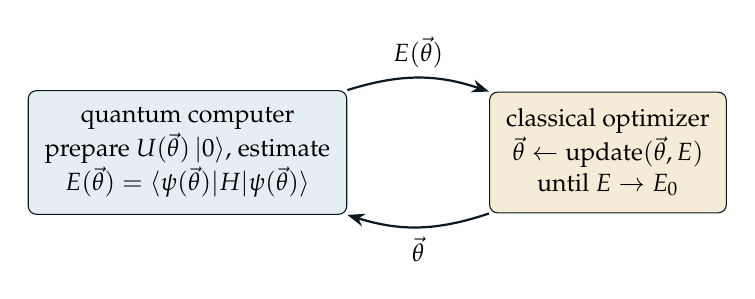
\begin{tikzpicture}
\node[box] (q) {quantum computer\\ prepare $U(\vec\theta)\ket{0}$, estimate\\ $E(\vec\theta)=\langle\psi(\vec\theta)|H|\psi(\vec\theta)\rangle$};
\node[box,fill=qxsand,right=1.8cm of q] (c) {classical optimizer\\ $\vec\theta\leftarrow\mathrm{update}(\vec\theta,E)$\\ until $E\to E_0$};
\draw[arr] (q.north east) to[bend left=18] node[above,font=\small]{$E(\vec\theta)$} (c.north west);
\draw[arr] (c.south west) to[bend left=18] node[below,font=\small]{$\vec\theta$} (q.south east);
\end{tikzpicture}
\end{tabular}

\end{document}
